In this section we will go over the results of the various experiments we have concocted. The results will be evaluated in two separate ways. For each experiment there are two models, the "final" model that was saved after all training was finished, and the "minloss" model which was saved during training when the model achieved the lowest loss. With the last experiment being the exception, all results shown are from the "final" models.\\

\noindent
The first evaluation will be on a structural classification dataset, which will be a qualitative analysis in which we perform t-distributed stochastic neighbor embedding (TSNE) dimensionality reduction on the data, and see whether it is able to cleanly separate the different types of protein structures. TSNE is preferred here over something like principal component analysis (PCA) due to this non-linearity of the reduction. This evaluation will be performed on the structural classification dataset. While using a classification method like k-nearest neighbors (KNN) might seem intuitive to quantitatively evaluate this, the non-linearity means that neither distance nor density is preserved between data points. We will also look at the next token prediction accuracy for the LSTM, but because we want to quantify how well it represents the proteins, this is not necessarily a good way to do that. It will mostly be used for comparison to see if there are any interesting insights.\\


\noindent
The second evaluation will be on the stability dataset. This evaluation will be quantitative, using Spearman's rank correlation coefficent. This coefficient measures the degree to which the relationship between two inputs can be described using a monotonic function. This means that having a high spearman correlation is equivalent to having a highly descriptive representation. It does not necessarily mean that the linear regression model we have trained provides good results in and of itself, since the coefficient does not describe a 1:1 correlation. This can be seen in figure ~\ref{fig:spearman}.

\begin{figure}[!ht]
  \centering
  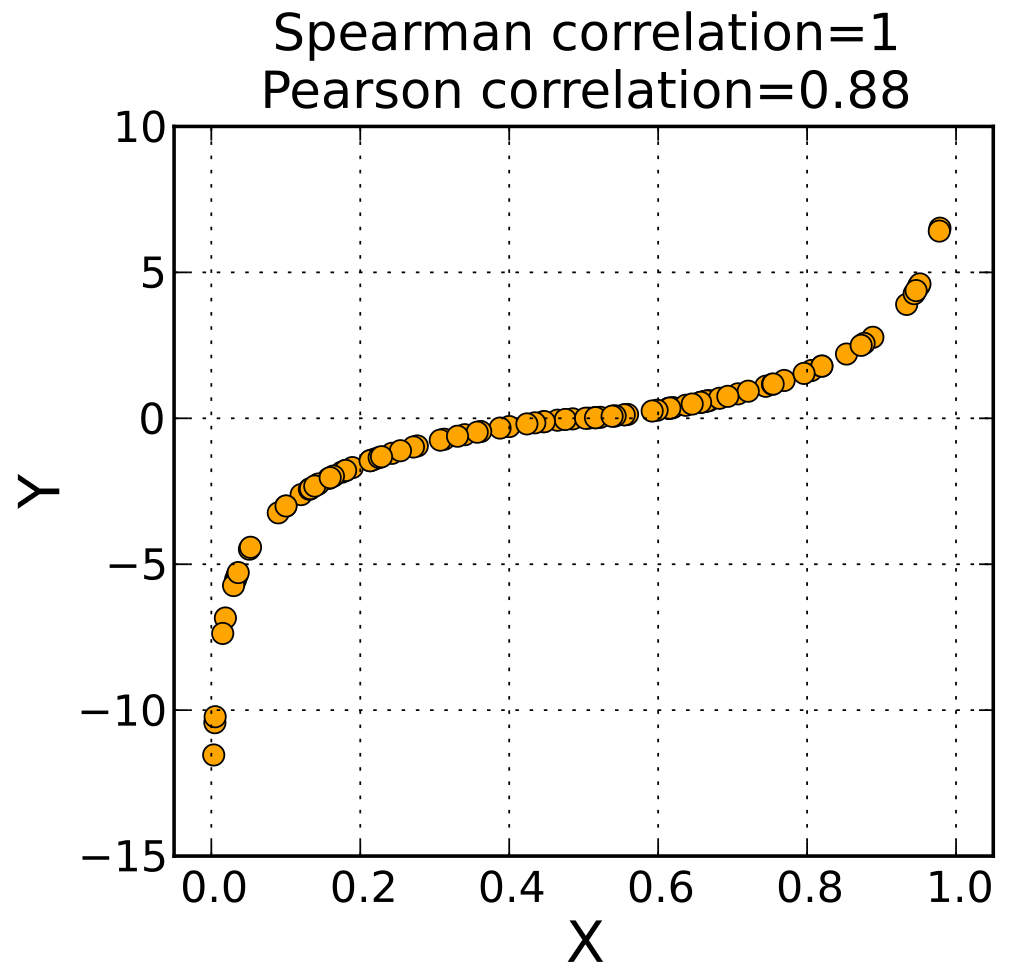
\includegraphics[width=0.4\linewidth]{latex/imgs/spearman_fig.png}
  \caption{Graph showing that high spearman correlation does not necessarily mean a good score. Image source:\cite{spearman}}\label{fig:spearman}
\end{figure}

\subsection{LSTM experiments}

\subsubsection{Layers vs no layers}
\begin{figure}[h]
	% Accuracy on test set: 12.43%, loss 2.84
  	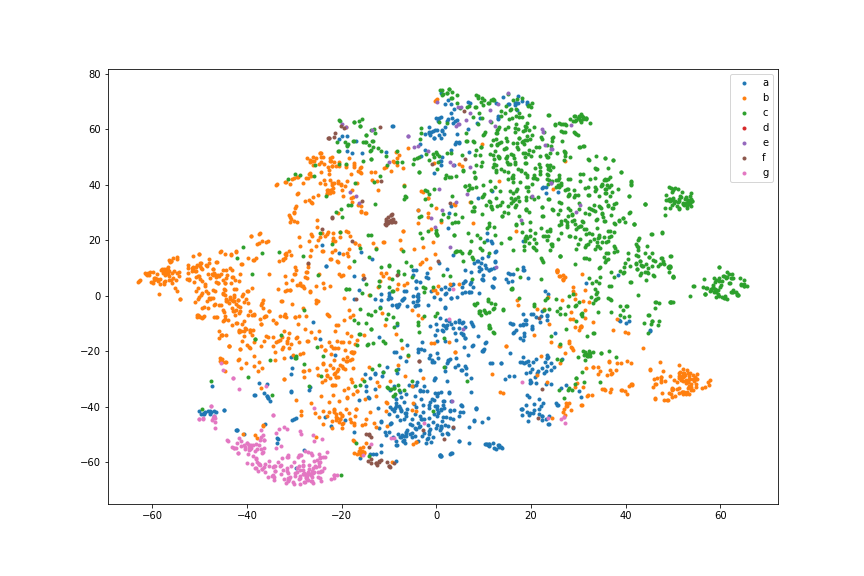
\includegraphics[width=0.4\linewidth]{latex/imgs/tsne_1_layer_with_schedule_512_final.png}
  	% Accuracy on test set: 13.03%, loss 2.83
  	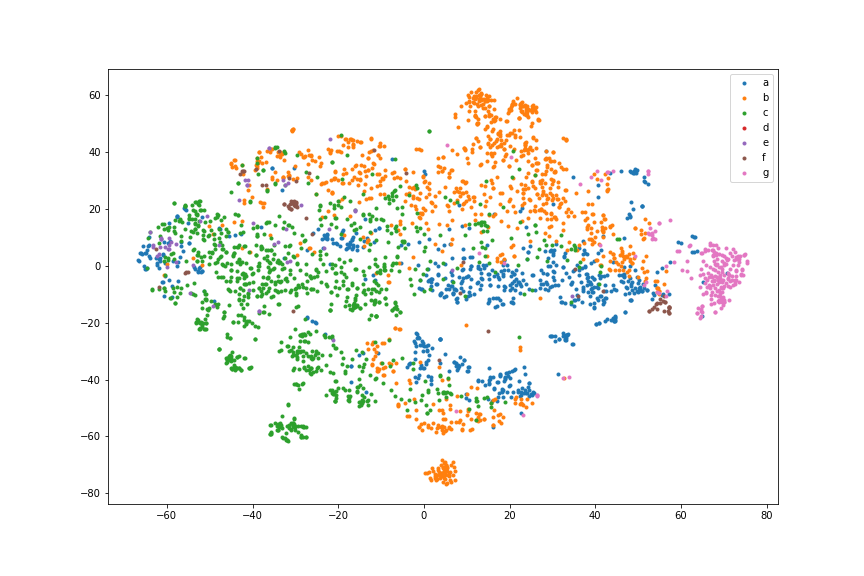
\includegraphics[width=0.4\linewidth]{latex/imgs/tsne_2_layer_no_drop_final.png}
	\caption{TSNE dimensionality reduction of the two models. Left is 1-layer, right is 2-layer}
\end{figure}

\begin{figure}[h]
	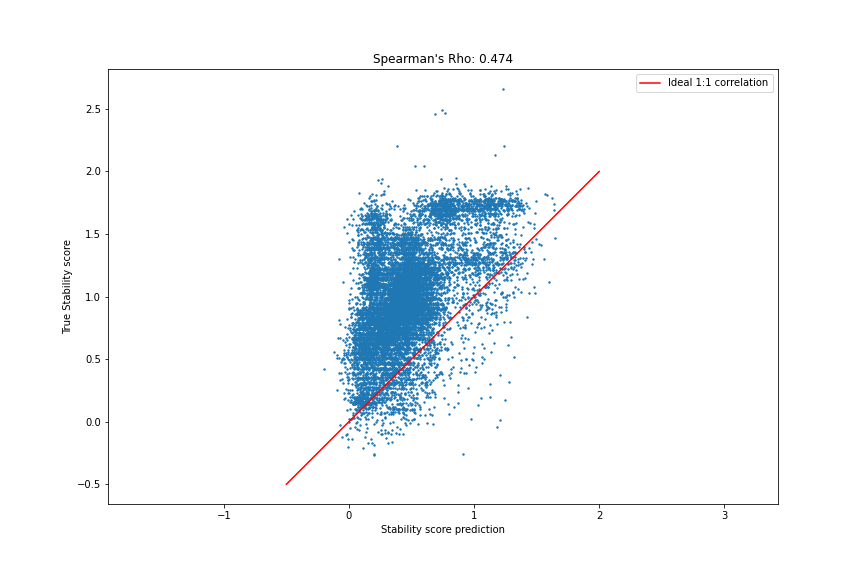
\includegraphics[width=0.4\linewidth]{latex/imgs/spearman_1_layer_with_schedule_512_final.png}
	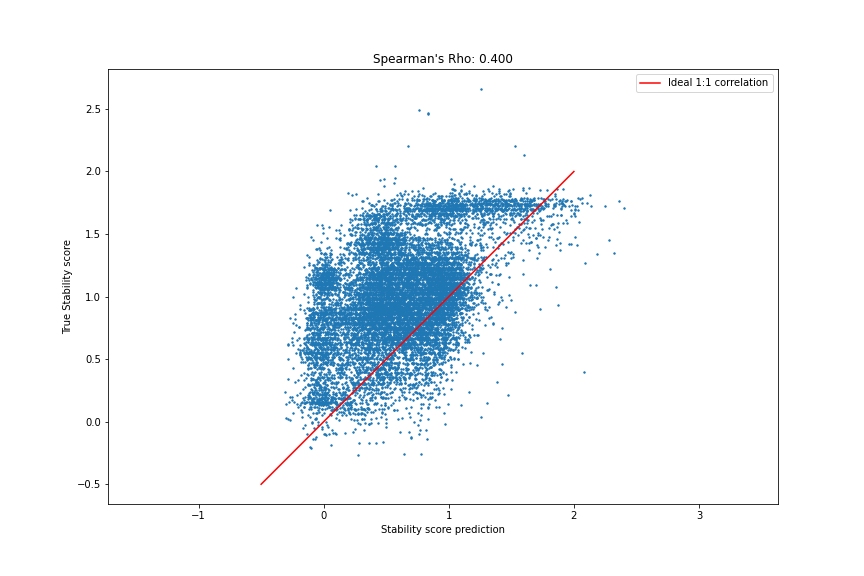
\includegraphics[width=0.4\linewidth]{latex/imgs/spearman_2_layer_no_drop_final.png}
	\caption{Plots used to calculate the Spearman correlation. Left is 1-layer, right is 2-layer}
\end{figure}

\begin{table}[]
\begin{tabular}{|l|l|l|l|}
\hline
        & Next token prediction accuracy & Test Loss & Spearman's rho\\ \hline
1-layer & 12.43\%                        & 2.84      & 0.400         \\ \hline
2-layer & 13.03\%                        & 2.83      & 0.428         \\ \hline
\end{tabular}
\end{table}

\subsubsection{Dropout vs no dropout}
\begin{figure}[!ht]
  \centering
  % Accuracy on test set: 13.03%, loss 2.83
  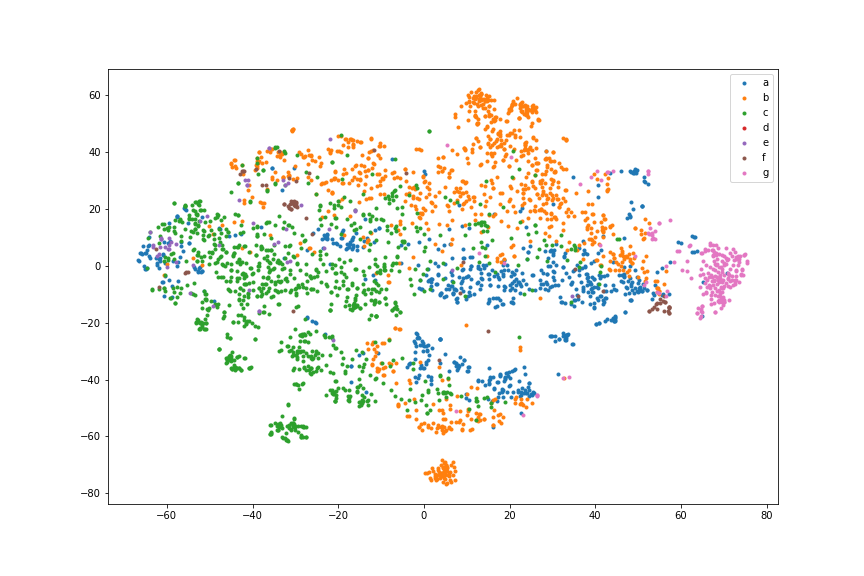
\includegraphics[width=0.49\linewidth]{latex/imgs/tsne_2_layer_no_drop_final.png}
  % Accuracy on test set: 13.02%, loss 2.82
  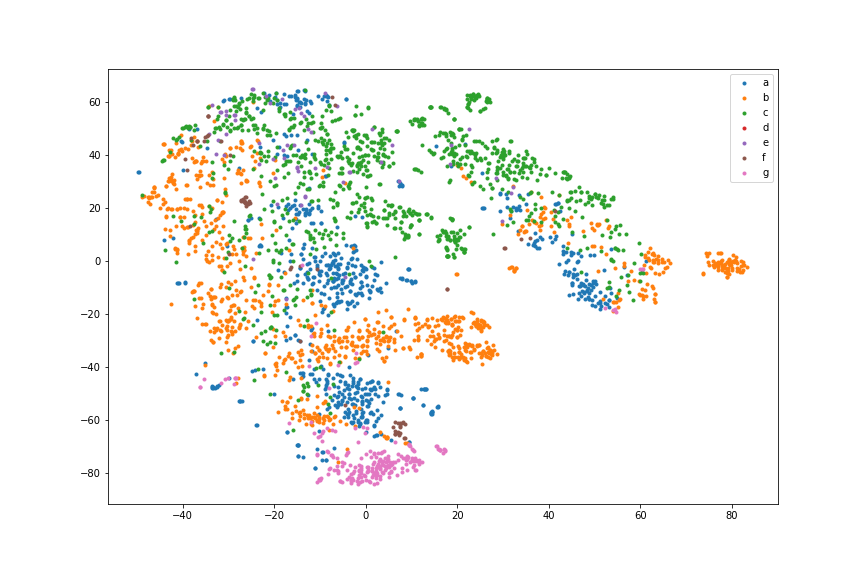
\includegraphics[width=0.49\linewidth]{latex/imgs/tsne_2_layer_05_drop_final.png}
  % 0.400 and 0.427
  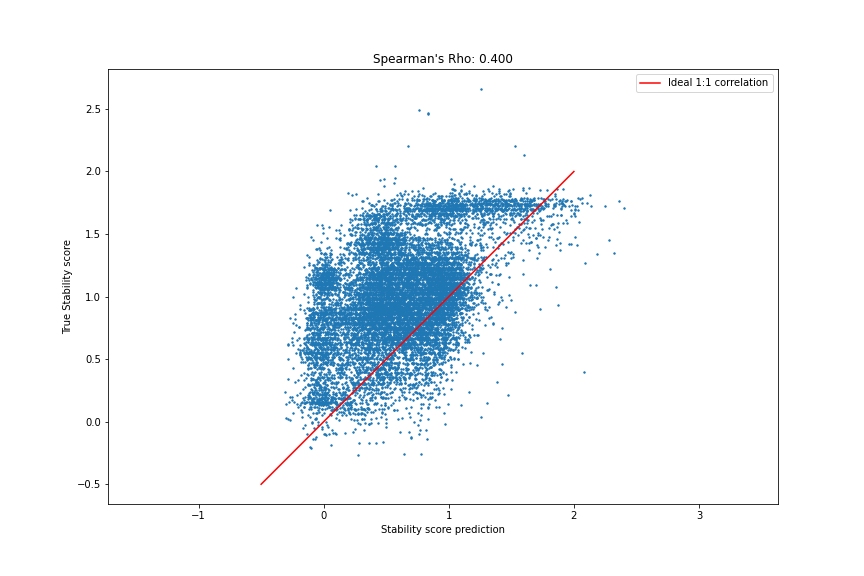
\includegraphics[width=0.49\linewidth]{latex/imgs/spearman_2_layer_no_drop_final.png}
  % 0.518 and 0.539
  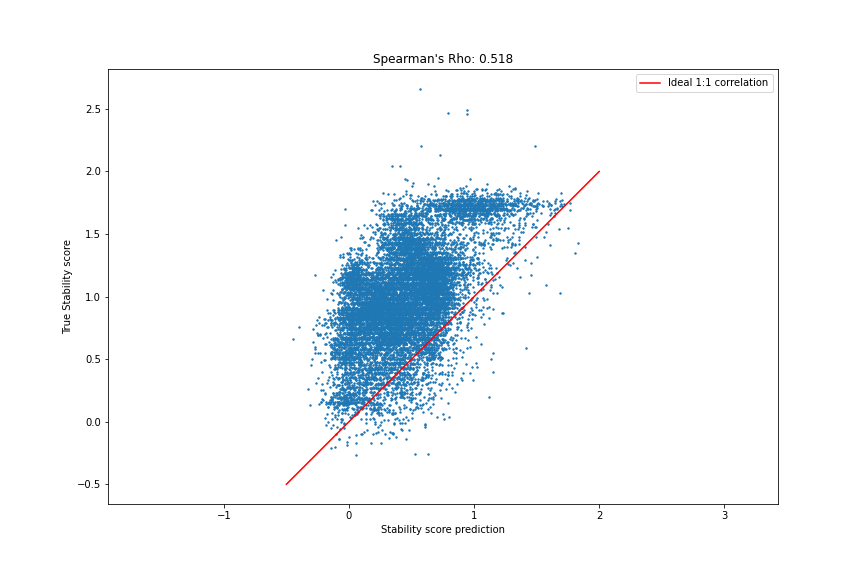
\includegraphics[width=0.49\linewidth]{latex/imgs/spearman_2_layer_05_drop_final.png}
  \caption{TSNE dimensionality reduction  and Spearman's rho data plots of the two models. Left is without dropout, right is with $50\%$ dropout.}
  \label{fig:cluster_spearman}
\end{figure}

\begin{table}[!ht]
\begin{tabular}{|l|l|l|l|}
\hline
             & Next token prediction accuracy & Test Loss & Spearman's rho\\ \hline
No dropout   & 13.03\%                        & 2.83      & 0.400         \\ \hline
50\% dropout & 13.02\%                        & 2.82      & 0.518         \\ \hline
\end{tabular}
\end{table}

\subsubsection{Feature size}
The feature size is the hyperparameter which controls the size of the internal layers of the LSTM. Increasing this should mean that the network can learn more complex functions. However, it also increases training time in a linear way. The increase is linear because for every feature you add, you have to backpropagate through one more. For this experiment we've trained three models with the following identical hyperparameters:
\begin{itemize}
	\item Layers: $1$
	\item Character embedding size: 30
	\item Starting learning rate: $8e-4$
	\item Learning rate schedule: Multiply by $0.2$ every 5 epochs
	\item Training time: 6 hours
\end{itemize}
The only difference between the models is the hidden layer size or feature size. We trained three models, one with $128$ features, one with $256$ features and one with $512$ features. Since training time is the most sparse resource for us, we decided that we would compare the results for equal real-time training time, not the number of epochs as with the other experiments.\\

\noindent
For this experiment we expect there to be some middle ground between the size of the model and how well it learns the representation. Since protein structures are very complex, we hypothesise that the larger models will perform better, even though they are not able to train for as many epochs.

\subsubsection{Learning Rate}
\begin{figure}[!ht]
  \centering
  % Accuracy on test set: 13.34%, loss 2.83
  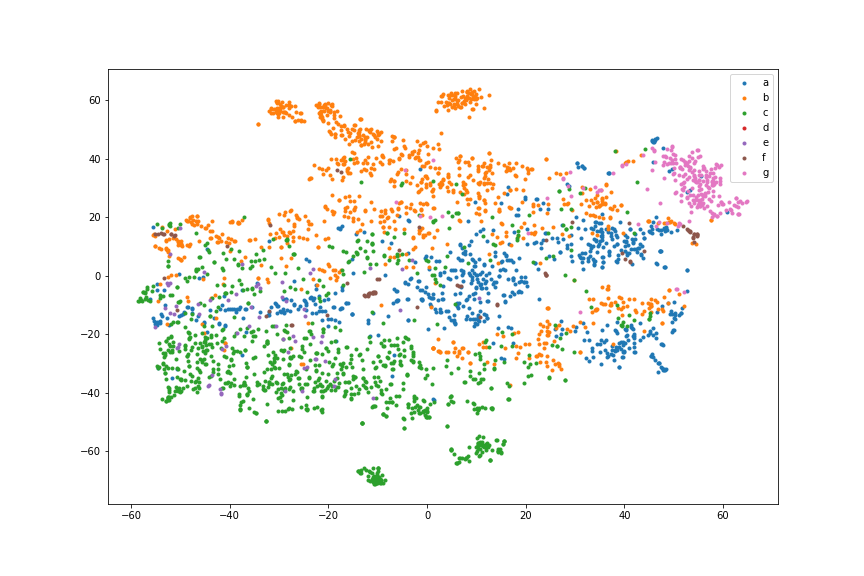
\includegraphics[width=0.49\linewidth]{latex/imgs/tsne_1_layer_no_schedule_512_final.png}
  % Accuracy on test set: 12.43%, loss 2.84
  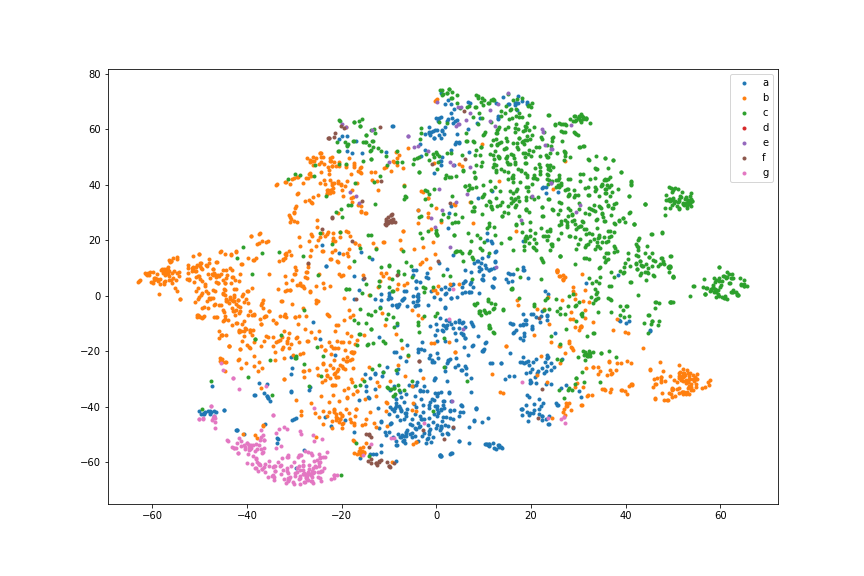
\includegraphics[width=0.49\linewidth]{latex/imgs/tsne_1_layer_with_schedule_512_final.png}
  % 0.605 and 0.592
  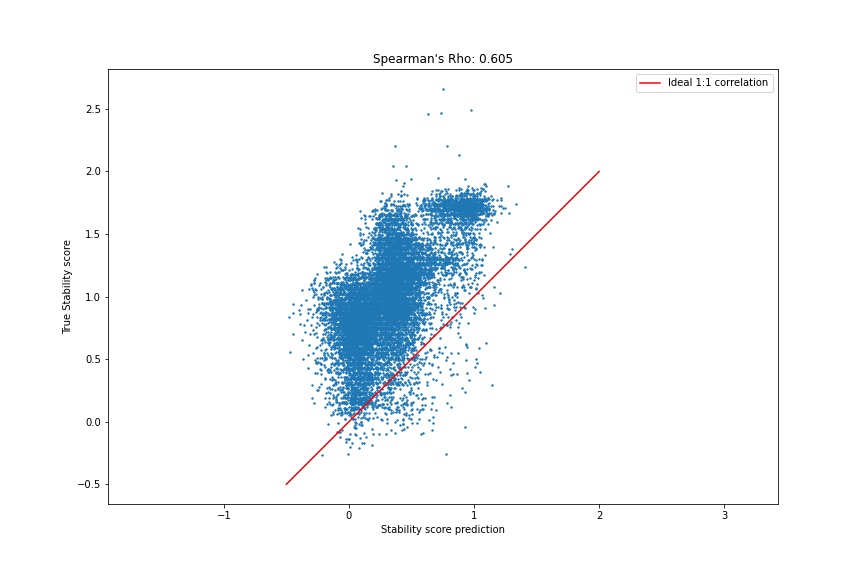
\includegraphics[width=0.49\linewidth]{latex/imgs/spearman_1_layer_no_schedule_512_final.png}
  % 0.428 and 0.414
  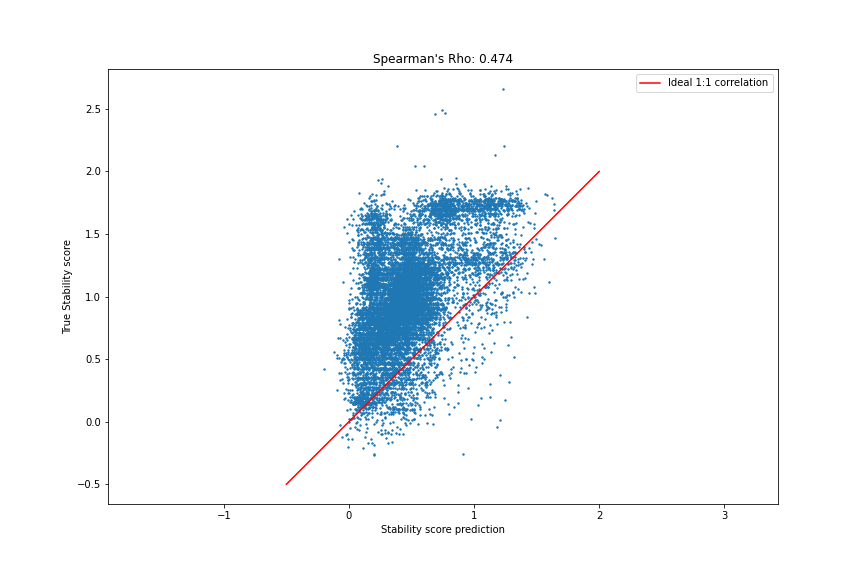
\includegraphics[width=0.49\linewidth]{latex/imgs/spearman_1_layer_with_schedule_512_final.png}
  \caption{TSNE dimensionality reduction  and Spearman's rho data plots of the two models. Left is without no learning rate schedule, right is with the schedule mention in the experiments section.}
\end{figure}

\begin{table}[!ht]
\begin{tabular}{|l|l|l|l|}
\hline
              & Next token prediction accuracy & Test Loss & Spearman's rho\\ \hline
No schedule   & 13.34\%                        & 2.83      & 0.605         \\ \hline
With schedule & 12.43\%                        & 2.84      & 0.474         \\ \hline
\end{tabular}
\end{table}

\subsubsection{Minimum loss model vs last model} % Finished
For this experiment we will not include the TSNE plots.
\begin{figure}[!ht]
  \centering
  % 0.518 and 0.539
  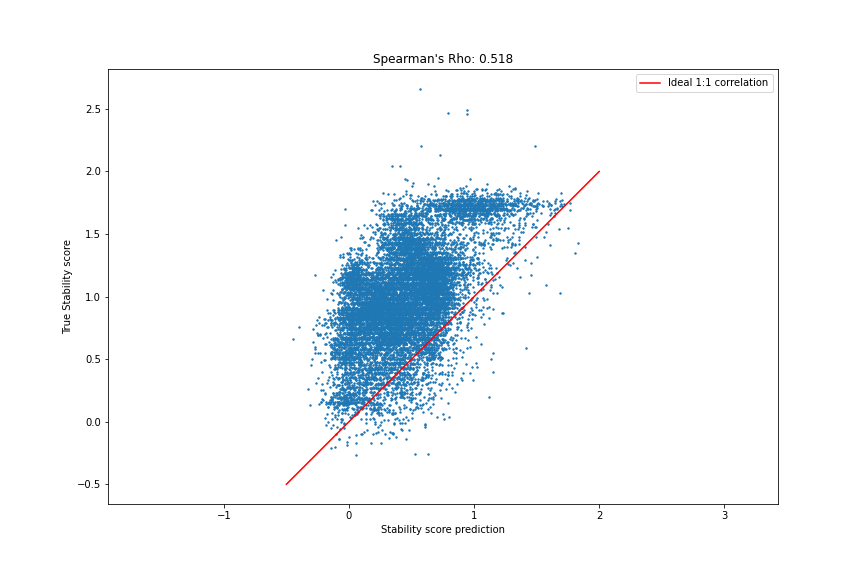
\includegraphics[width=0.49\linewidth]{latex/imgs/spearman_2_layer_05_drop_final.png}
  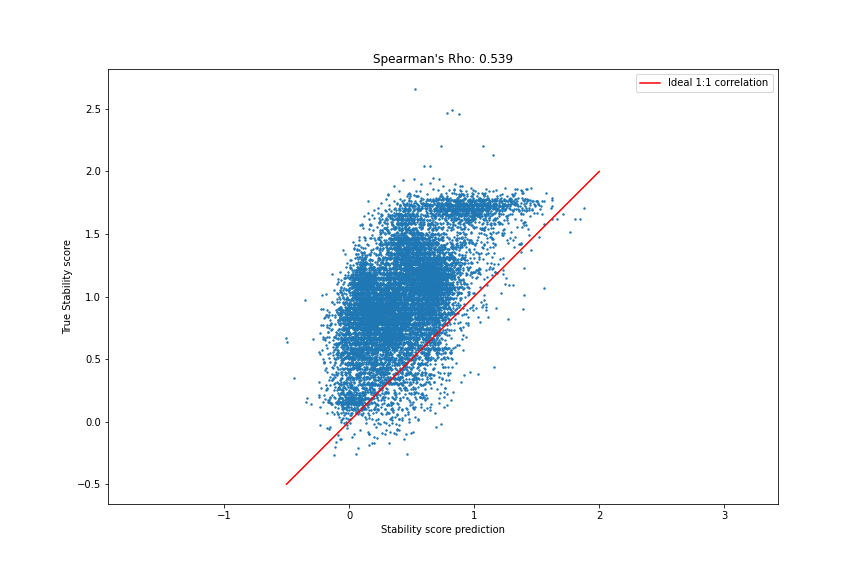
\includegraphics[width=0.49\linewidth]{latex/imgs/spearman_2_layer_05_drop_minloss.png}
  % 0.400 and 0.427
  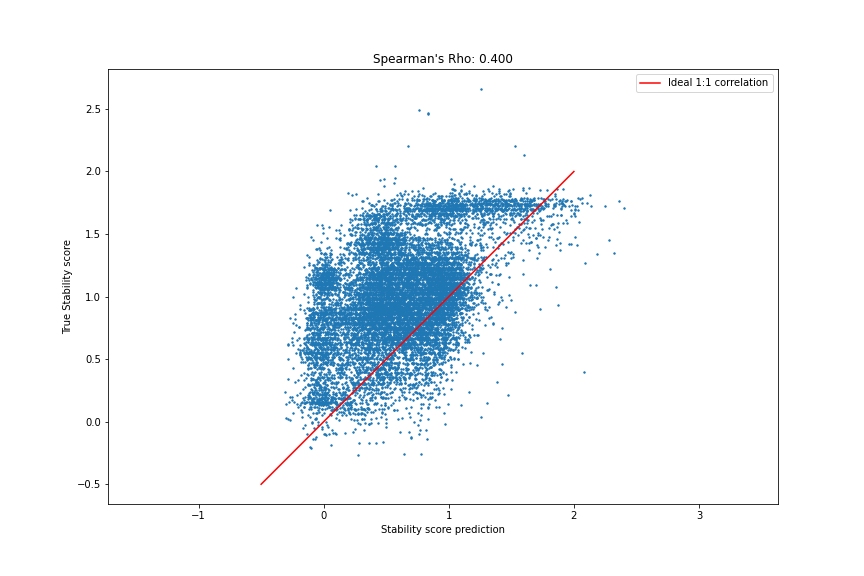
\includegraphics[width=0.49\linewidth]{latex/imgs/spearman_2_layer_no_drop_final.png}
  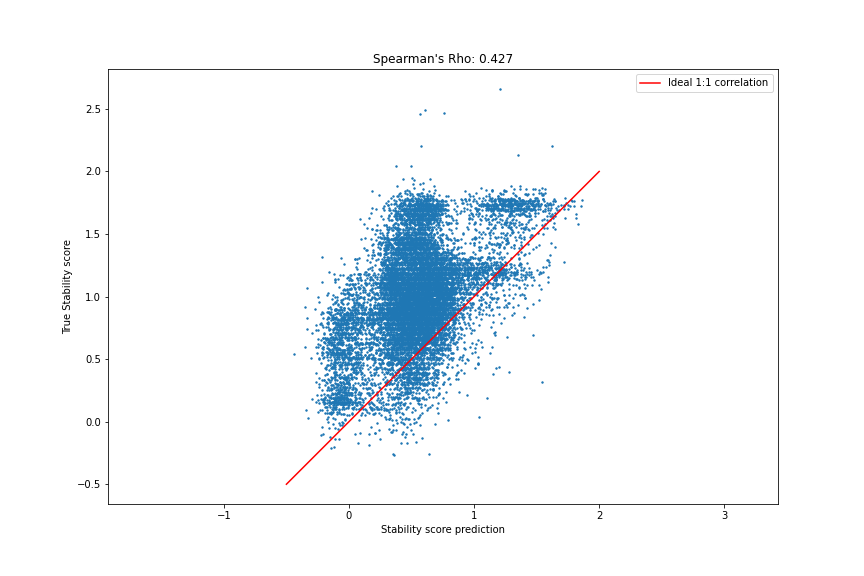
\includegraphics[width=0.49\linewidth]{latex/imgs/spearman_2_layer_no_drop_minloss.png}
  % 0.605 and 0.592
  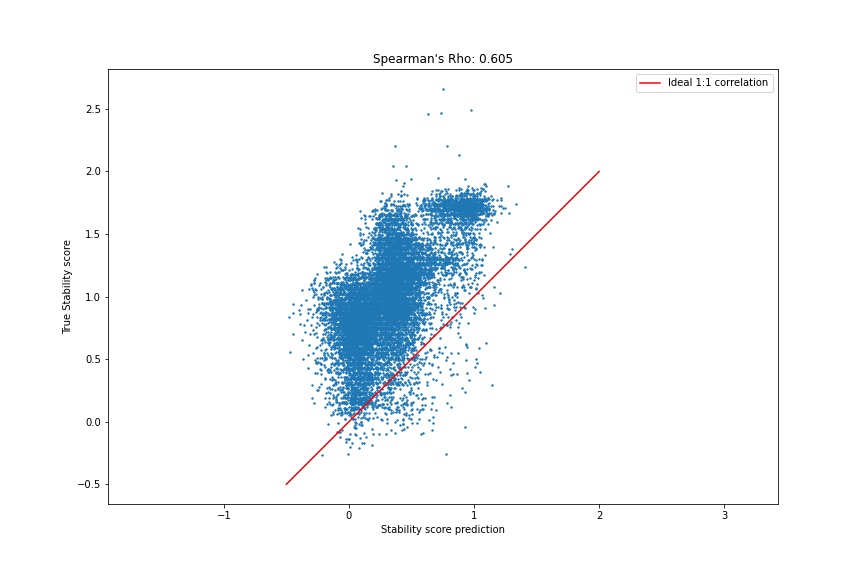
\includegraphics[width=0.49\linewidth]{latex/imgs/spearman_1_layer_no_schedule_512_final.png}
  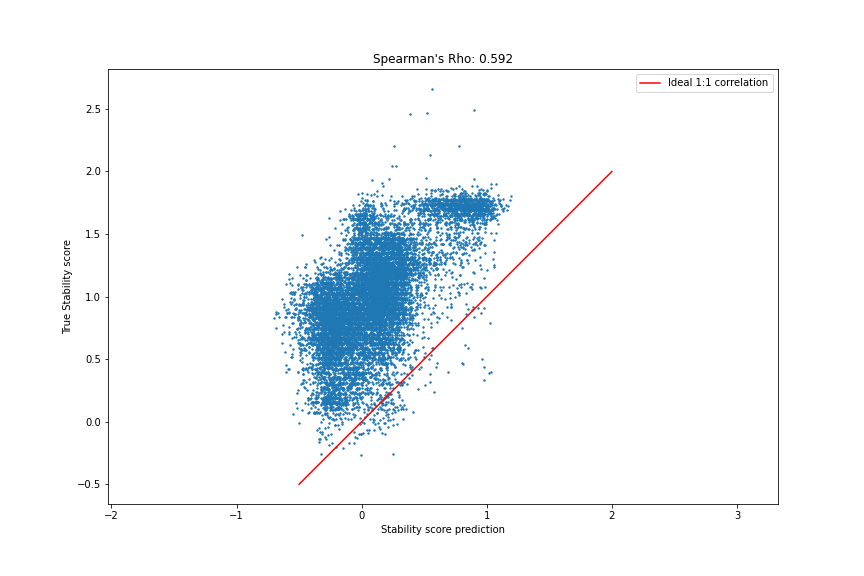
\includegraphics[width=0.49\linewidth]{latex/imgs/spearman_1_layer_no_schedule_512_minloss.png}
  % 0.428 and 0.414
  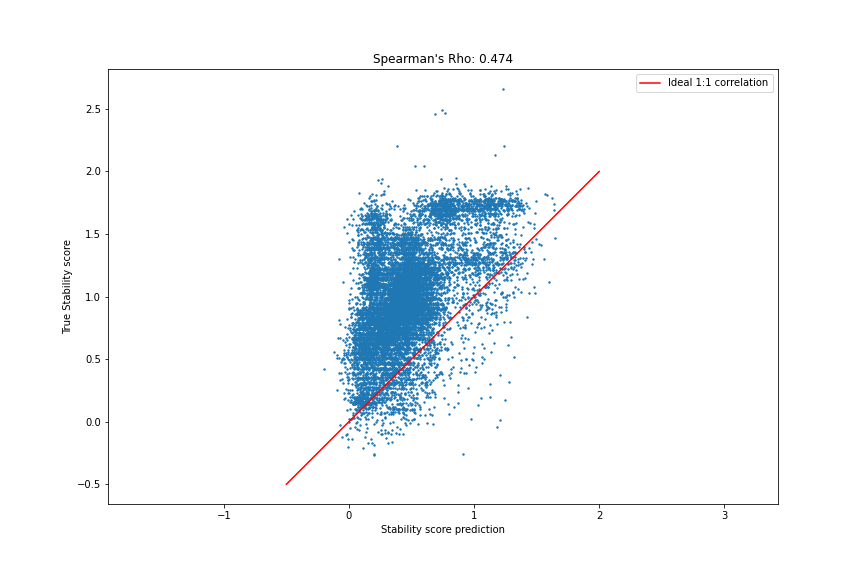
\includegraphics[width=0.49\linewidth]{latex/imgs/spearman_1_layer_with_schedule_512_final.png}
  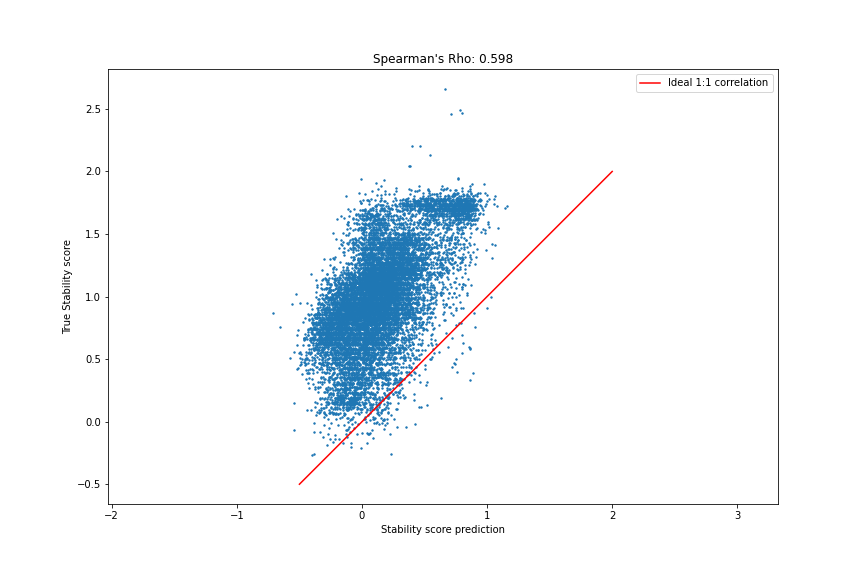
\includegraphics[width=0.49\linewidth]{latex/imgs/spearman_1_layer_with_schedule_512_minloss.png}
  % 0.435 and 0.424
  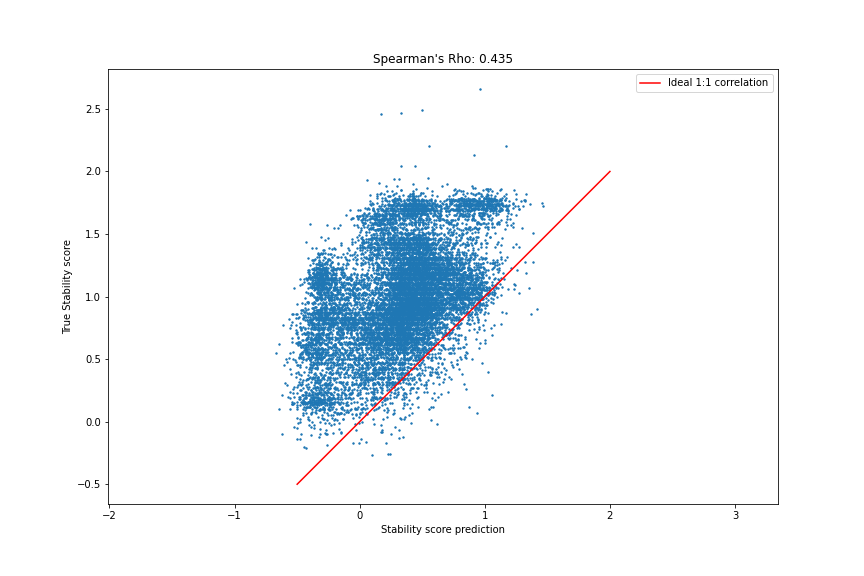
\includegraphics[width=0.49\linewidth]{latex/imgs/spearman_1_layer_with_schedule_256_final.png}
  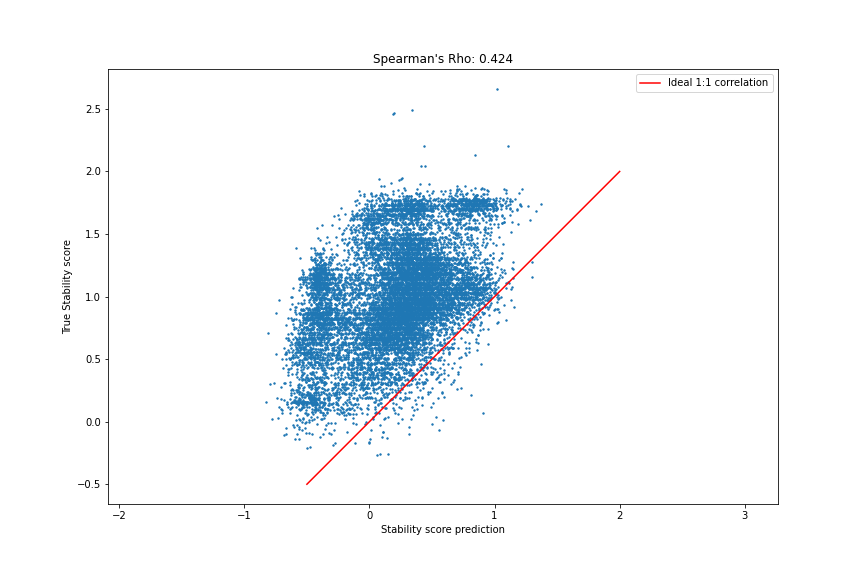
\includegraphics[width=0.49\linewidth]{latex/imgs/spearman_1_layer_with_schedule_256_minloss.png}
  % 0.507 and 0.627
  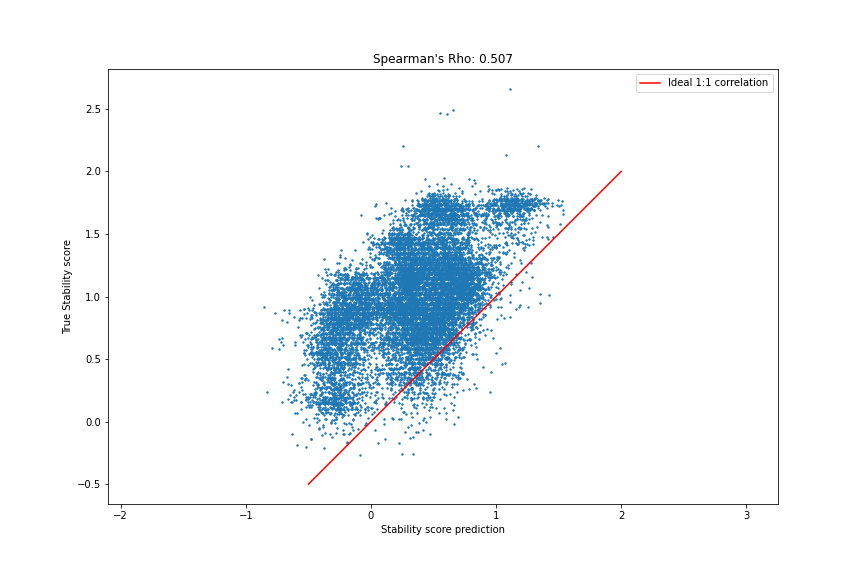
\includegraphics[width=0.49\linewidth]{latex/imgs/spearman_1_layer_with_schedule_1024_final.png}
  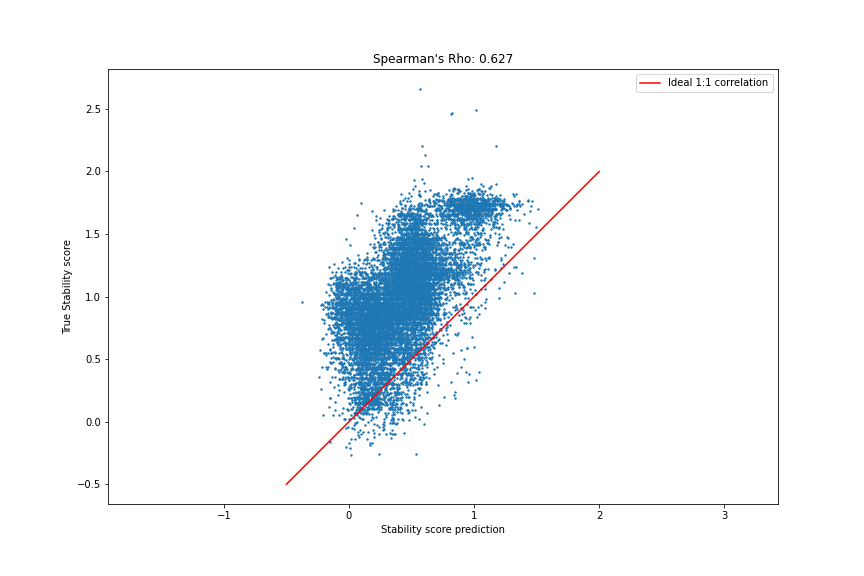
\includegraphics[width=0.49\linewidth]{latex/imgs/spearman_1_layer_with_schedule_1024_minloss.png}
  \caption{TSNE dimensionality reduction  and Spearman's rho data plots of the two models. Left is without no learning rate schedule, right is with the schedule mention in the experiments section.}
\end{figure}

\begin{table}[!ht]
\begin{tabular}{|l|lll|}
\hline
                                      &                                                     & Final Models                       &                \\ \cline{2-4} 
                                      & \multicolumn{1}{l|}{Next token prediction accuracy} & \multicolumn{1}{l|}{Test Loss}     & Spearman's rho \\ \hline
2-layer, 50\% dropout, 512 features   & \multicolumn{1}{l|}{13.02\%}                        & \multicolumn{1}{l|}{2.82}          & 0.518          \\ \hline
2-layer, no dropout, 512 features     & \multicolumn{1}{l|}{13.03\%}                        & \multicolumn{1}{l|}{2.83}          & 0.400          \\ \hline
1-layer, no lr schedule, 512 features & \multicolumn{1}{l|}{13.34\%}                        & \multicolumn{1}{l|}{2.83}          & \textbf{0.605} \\ \hline
1-layer, 256 features                 & \multicolumn{1}{l|}{11.41\%}                        & \multicolumn{1}{l|}{2.86}          & 0.435          \\ \hline
1-layer, 512 features                 & \multicolumn{1}{l|}{12.43\%}                        & \multicolumn{1}{l|}{2.84}          & 0.428          \\ \hline
1-layer, 1024 features                & \multicolumn{1}{l|}{\textbf{14.37\%}}               & \multicolumn{1}{l|}{\textbf{2.79}} & 0.507          \\ \hline
\end{tabular}
\end{table}
\begin{table}[!ht]
\begin{tabular}{|l|lll|}
\hline
                                      &                                                     & Minloss models                     &                \\ \cline{2-4} 
                                      & \multicolumn{1}{l|}{Next token prediction accuracy} & \multicolumn{1}{l|}{Test Loss}     & Spearman's rho \\ \hline
2-layer, 50\% dropout, 512 features   & \multicolumn{1}{l|}{13.03\%}                        & \multicolumn{1}{l|}{2.82}          & 0.539          \\ \hline
2-layer, no dropout, 512 features     & \multicolumn{1}{l|}{13.78\%}                        & \multicolumn{1}{l|}{2.81}          & 0.427          \\ \hline
1-layer, no lr schedule, 512 features & \multicolumn{1}{l|}{13.36\%}                        & \multicolumn{1}{l|}{2.83}          & 0.592          \\ \hline
1-layer, 256 features                 & \multicolumn{1}{l|}{11.40\%}                        & \multicolumn{1}{l|}{2.87}          & 0.424          \\ \hline
1-layer, 512 features                 & \multicolumn{1}{l|}{12.43\%}                        & \multicolumn{1}{l|}{2.85}          & 0.414          \\ \hline
1-layer, 1024 features                & \multicolumn{1}{l|}{\textbf{14.22\%}}               & \multicolumn{1}{l|}{\textbf{2.80}} & \textbf{0.627} \\ \hline
\end{tabular}
\end{table}

\subsubsection{CNN}
Training the model with different sizes of latent dimensions yielded some different results, in different aspects of the task the model had. Below can we see how the loss differ from each other: \\

\begin{figure}[!ht]
  \centering
  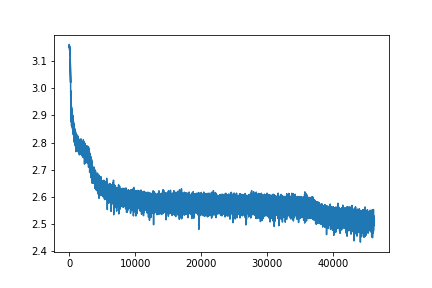
\includegraphics[width=0.4\linewidth]{latex/imgs/CNN_loss_latent_dimension_100.png}
  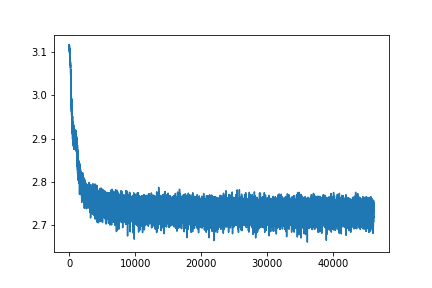
\includegraphics[width=0.4\linewidth]{latex/imgs/loss_latent_dimension_50.png}
  \caption{losses of the of cnn trained with latent dimension $4$x$100$(left) and $2$x$50$(right)}
  \label{fig:cnn_loss}
\end{figure}

\noindent
As can be seen on the graph (figure ~\ref{fig:cnn_loss}), the one with a high latent dimension had a noticeably better loss, than the one with a lower latent dimension. Which makes good sense, since the model with a greater latent dimension has more data to use in the reconstruction. Since the loss was based on the model's ability to reconstruct the image; it is no surprise that the one with higher dimensionality reduction, had better reconstruction accuracy.

\begin{table}[!ht]
\centering
\begin{tabular}{|l|l|l|}
\hline
 latent\_dimension: & $4$x$100$  &  $2$x$50$ \\ \hline
min\_loss model     & 0.2039 & 0.1473 \\ \hline
fully trained model & 0.2058 & 0.1469 \\ \hline
\end{tabular}
\caption{reconstruction accuracy}
\end{table}

\noindent
It's important to note, that the reconstruction accuracy is not defining how well the model is performing on the separation task or the spearmen correlation.\\

\noindent
The following figures (figure ~\ref{fig:plot_50} and ~\ref{fig:plot_100}) show the structural plotting of the model's latent representation run through a t-sne. As can be seen, on the figures. The model seems to find some separation between the different structural classes. As can be seen, both models find some separation between classes (C, B, G) with some overlapping. The rest of the classes is mostly spread out between the groups. Indicating that this model is not very good at finding much structural separation. \\

\begin{figure}[!ht]
  \centering
  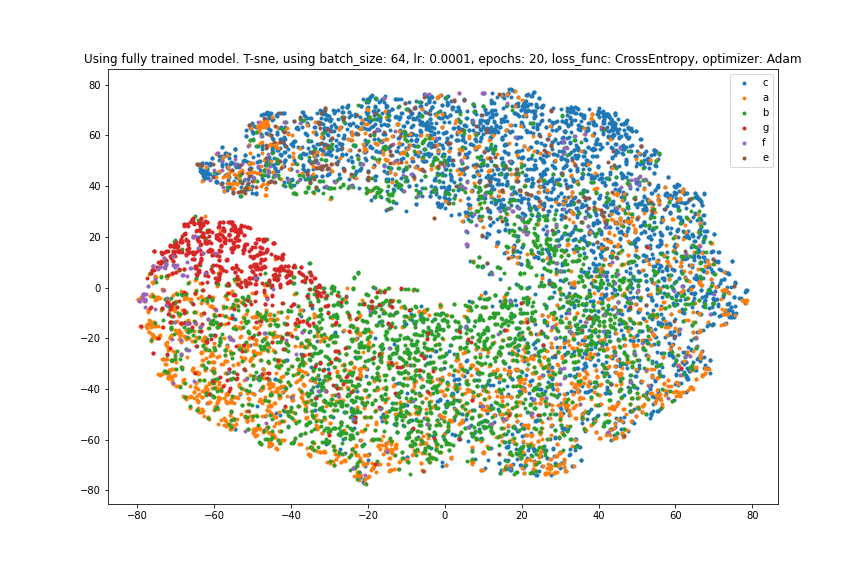
\includegraphics[width=0.4\linewidth]{latex/imgs/last_50.png}
  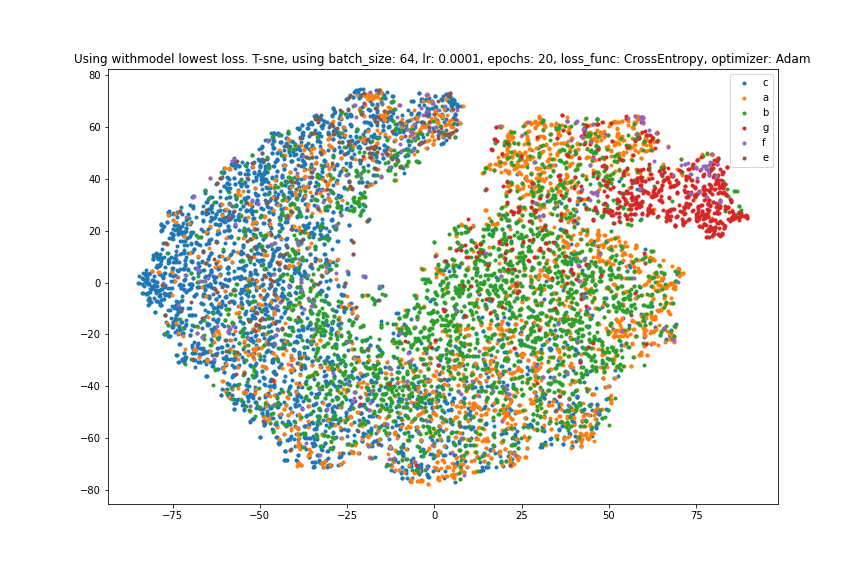
\includegraphics[width=0.4\linewidth]{latex/imgs/best_50.png}
  \caption{plot showing secondary structure seperation with latent dimension $2$x$50$. Fully trained model(left), min loss model (left)}
  \label{fig:plot_50}
\end{figure}

\begin{figure}[!ht]
  \centering
  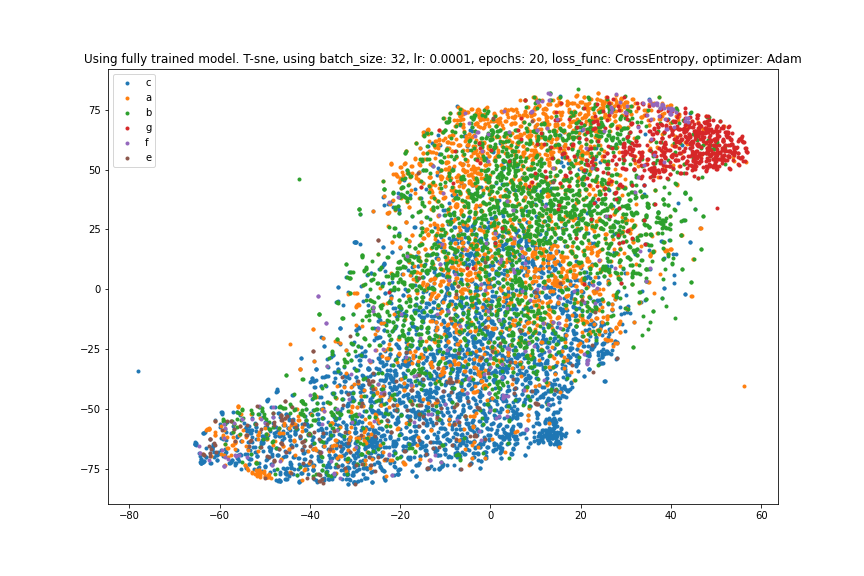
\includegraphics[width=0.4\linewidth]{latex/imgs/last_100.png}
  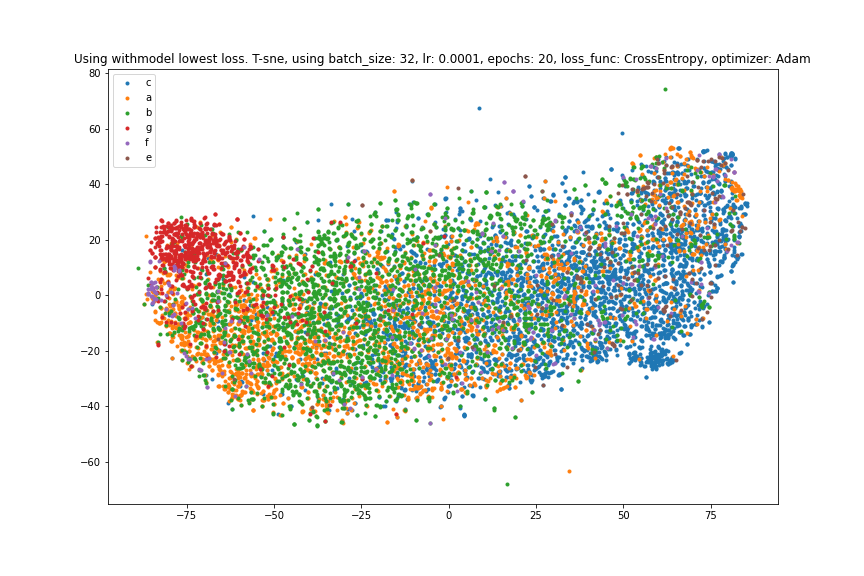
\includegraphics[width=0.4\linewidth]{latex/imgs/best_100.png}
  \caption{plot showing secondary structure seperation with latent dimension $4$x$100$. Fully trained model(left), min loss model (left)}
  \label{fig:plot_100}
\end{figure}

\noindent
The two figures (figure ~\ref{fig:stab_100} and ~\ref{fig:stab_50}) yielded the following results on the stability dataset calculating spearment correlation.


\begin{figure}[!ht]
  \centering
  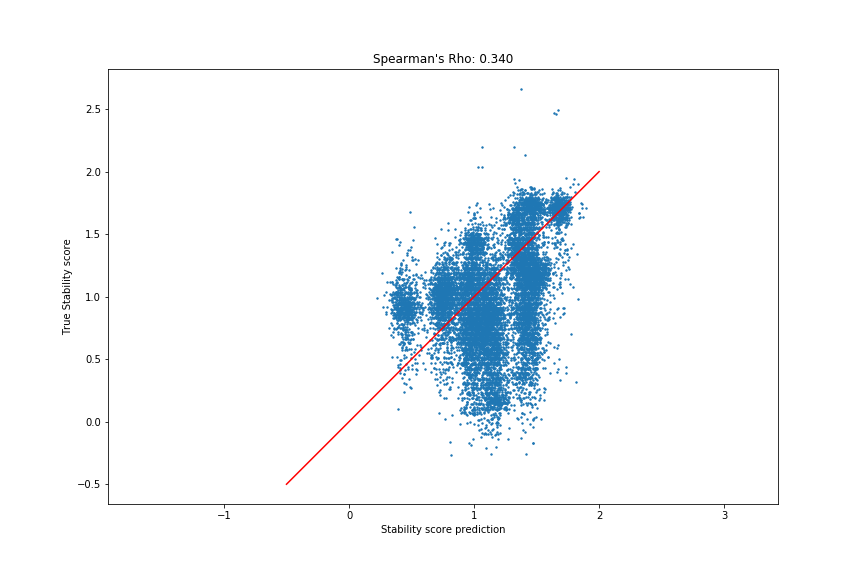
\includegraphics[width=0.4\linewidth]{latex/imgs/CNN_spearman_correlation_100_fully.png}
  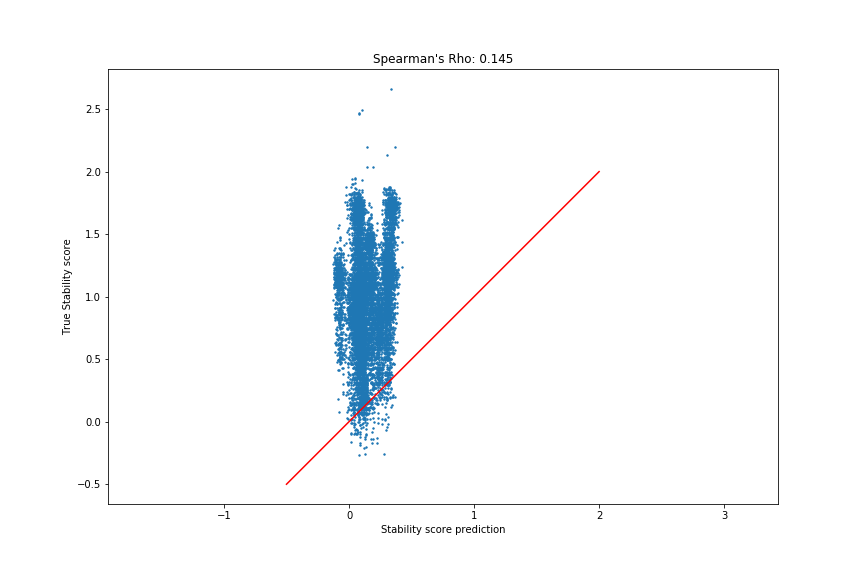
\includegraphics[width=0.4\linewidth]{latex/imgs/CNN_spearman_correlation_100_best.png}
  \caption{Graph showing the spearman correlation from model with latent dimension $4$x$100$. Fully trained model(left), min loss model (left)}
  \label{fig:stab_100}
\end{figure}

\begin{figure}[!ht]
  \centering
  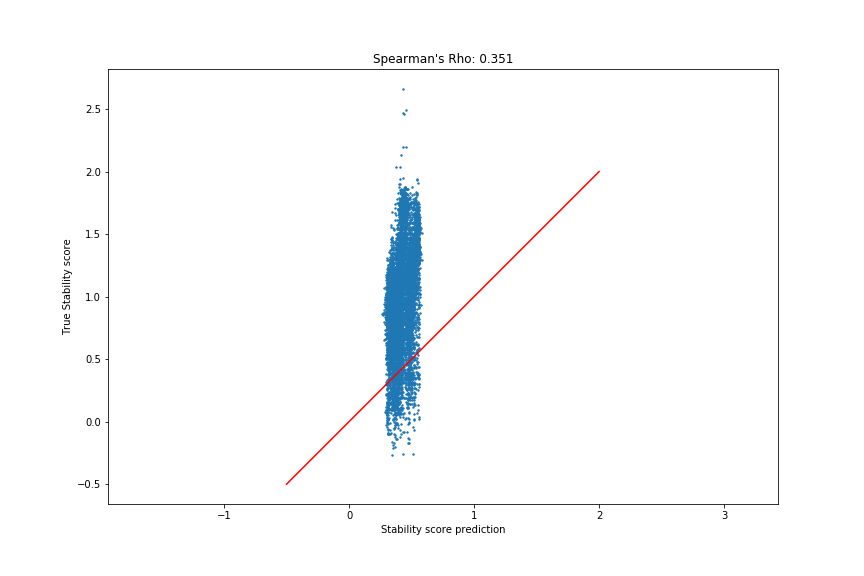
\includegraphics[width=0.4\linewidth]{latex/imgs/CNN_spearman_correlation_50_fully.png}
  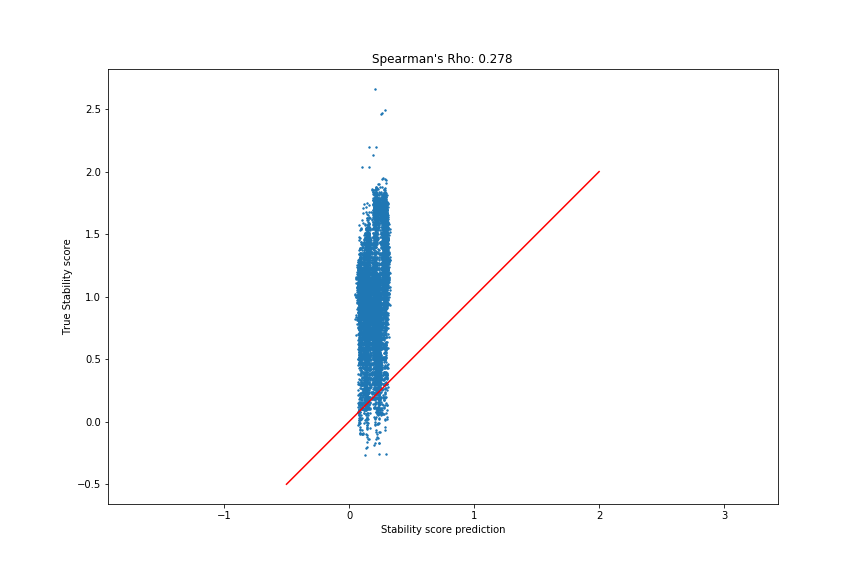
\includegraphics[width=0.4\linewidth]{latex/imgs/CNN_spearman_correlation_50_best.png}
  \caption{Graph showing the spearman correlation from model with latent dimension $2$x$50$. Fully trained model(left), min loss model (left)}
  \label{fig:stab_50}
\end{figure}

\noindent
It would seem that the model converges at about 0.3, which not especially great results since they are pretty far from the optimal results 1. Yet, it means that the model has learned some representation of the structure. \\

\noindent
In general in these experiments, the results from the minimum loss model, doesn't perform that different compared to the fully trained model.
